%% LaTeX-Beamer template for KIT design
%% by Erik Burger, Christian Hammer
%% title picture by Klaus Krogmann
%%
%% version 2.1
%%
%% mostly compatible to KIT corporate design v2.0
%% http://intranet.kit.edu/gestaltungsrichtlinien.php
%%
%% Problems, bugs and comments to
%% burger@kit.edu

\documentclass[18pt]{beamer}

%% SLIDE FORMAT

% use 'beamerthemekit' for standard 4:3 ratio
% for widescreen slides (16:9), use 'beamerthemekitwide'

\usepackage{templates/beamerthemekit}
\usepackage[utf8]{inputenc}
% \usepackage{templates/beamerthemekitwide}

\usepackage{graphicx}

%% TITLE PICTURE

% if a custom picture is to be used on the title page, copy it into the 'logos'
% directory, in the line below, replace 'mypicture' with the
% filename (without extension) and uncomment the following line
% (picture proportions: 63 : 20 for standard, 169 : 40 for wide
% *.eps format if you use latex+dvips+ps2pdf,
% *.jpg/*.png/*.pdf if you use pdflatex)

\titleimage{labor}

%% TITLE LOGO

% for a custom logo on the front page, copy your file into the 'logos'
% directory, insert the filename in the line below and uncomment it

\titlelogo{title}

% (*.eps format if you use latex+dvips+ps2pdf,
% *.jpg/*.png/*.pdf if you use pdflatex)

%% TikZ INTEGRATION

% use these packages for PCM symbols and UML classes
% \usepackage{templates/tikzkit}
% \usepackage{templates/tikzuml}

% the presentation starts here

\title[TruffleHog \& spp\_profinet]{TruffleHog \& spp\_profinet}
%\subtitle{2015}
\author{Maximilian Diez, Mark Giraud, Jan Hermes}

\institute{Fraunhofer IOSB}

% Bibliography

%\usepackage[citestyle=authoryear,bibstyle=numeric,hyperref,backend=biber]{biblatex}
%\addbibresource{templates/example.bib}
%\bibhang1em

\begin{document}

% change the following line to "ngerman" for German style date and logos
\selectlanguage{ngerman}

%title page
\begin{frame}
\titlepage
\end{frame}

%table of contents
%\begin{frame}{Gliederung}
%\tableofcontents
%\end{frame}

\section{Einleitung}
\begin{frame}{Einleitung: Motivation}
    \begin{itemize}
      \item PROFINET zur einfacheren Vernetzung von Industrieanlagen
      \pause
      \item Sicherheit im industriellen Kontext
      \pause
      \item Paketanalyse mit Snort
      \pause
      \item Visualisierung
      \only<4->{\begin{figure}
      	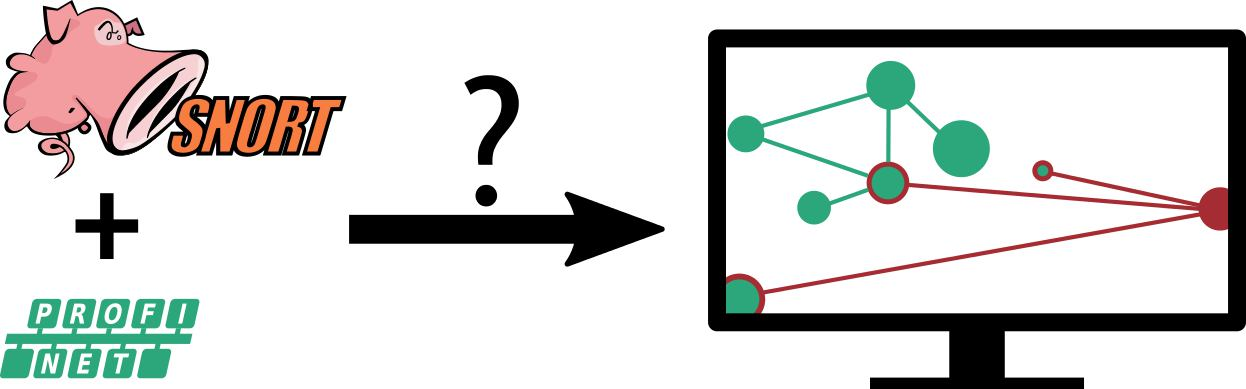
\includegraphics[width=0.9\textwidth]{./images/aufgabestellung.jpg}
      \end{figure}}
    \end{itemize}
\end{frame}

\begin{frame}{Einleitung: Plugin}
    \begin{itemize}
      \item Identifizierung und Dekodierung von PROFINET Paketen (Ethertyp 0x8892)
      \pause
      \item Bereitstellen von Verbindungsdaten für einen Klienten
      \pause
      \item Optional: Auslösen von Alerts in Snort zur automatisierten Überwachung
    \end{itemize}
\end{frame}


\begin{frame}{Einleitung: TruffleHog}
    \begin{itemize}
      \item Empfängt Verbindungsdaten
      \pause
      \item Verarbeitet Pakete und\dots
      \pause
      \begin{itemize}
        \item stellt Netzwerkteilnehmer als Knoten, \pause
        \item Verbindungen als Kanten dar. 
      \end{itemize}
    \end{itemize}
\end{frame}


\begin{frame}
    \begin{figure}
    	\centering
    	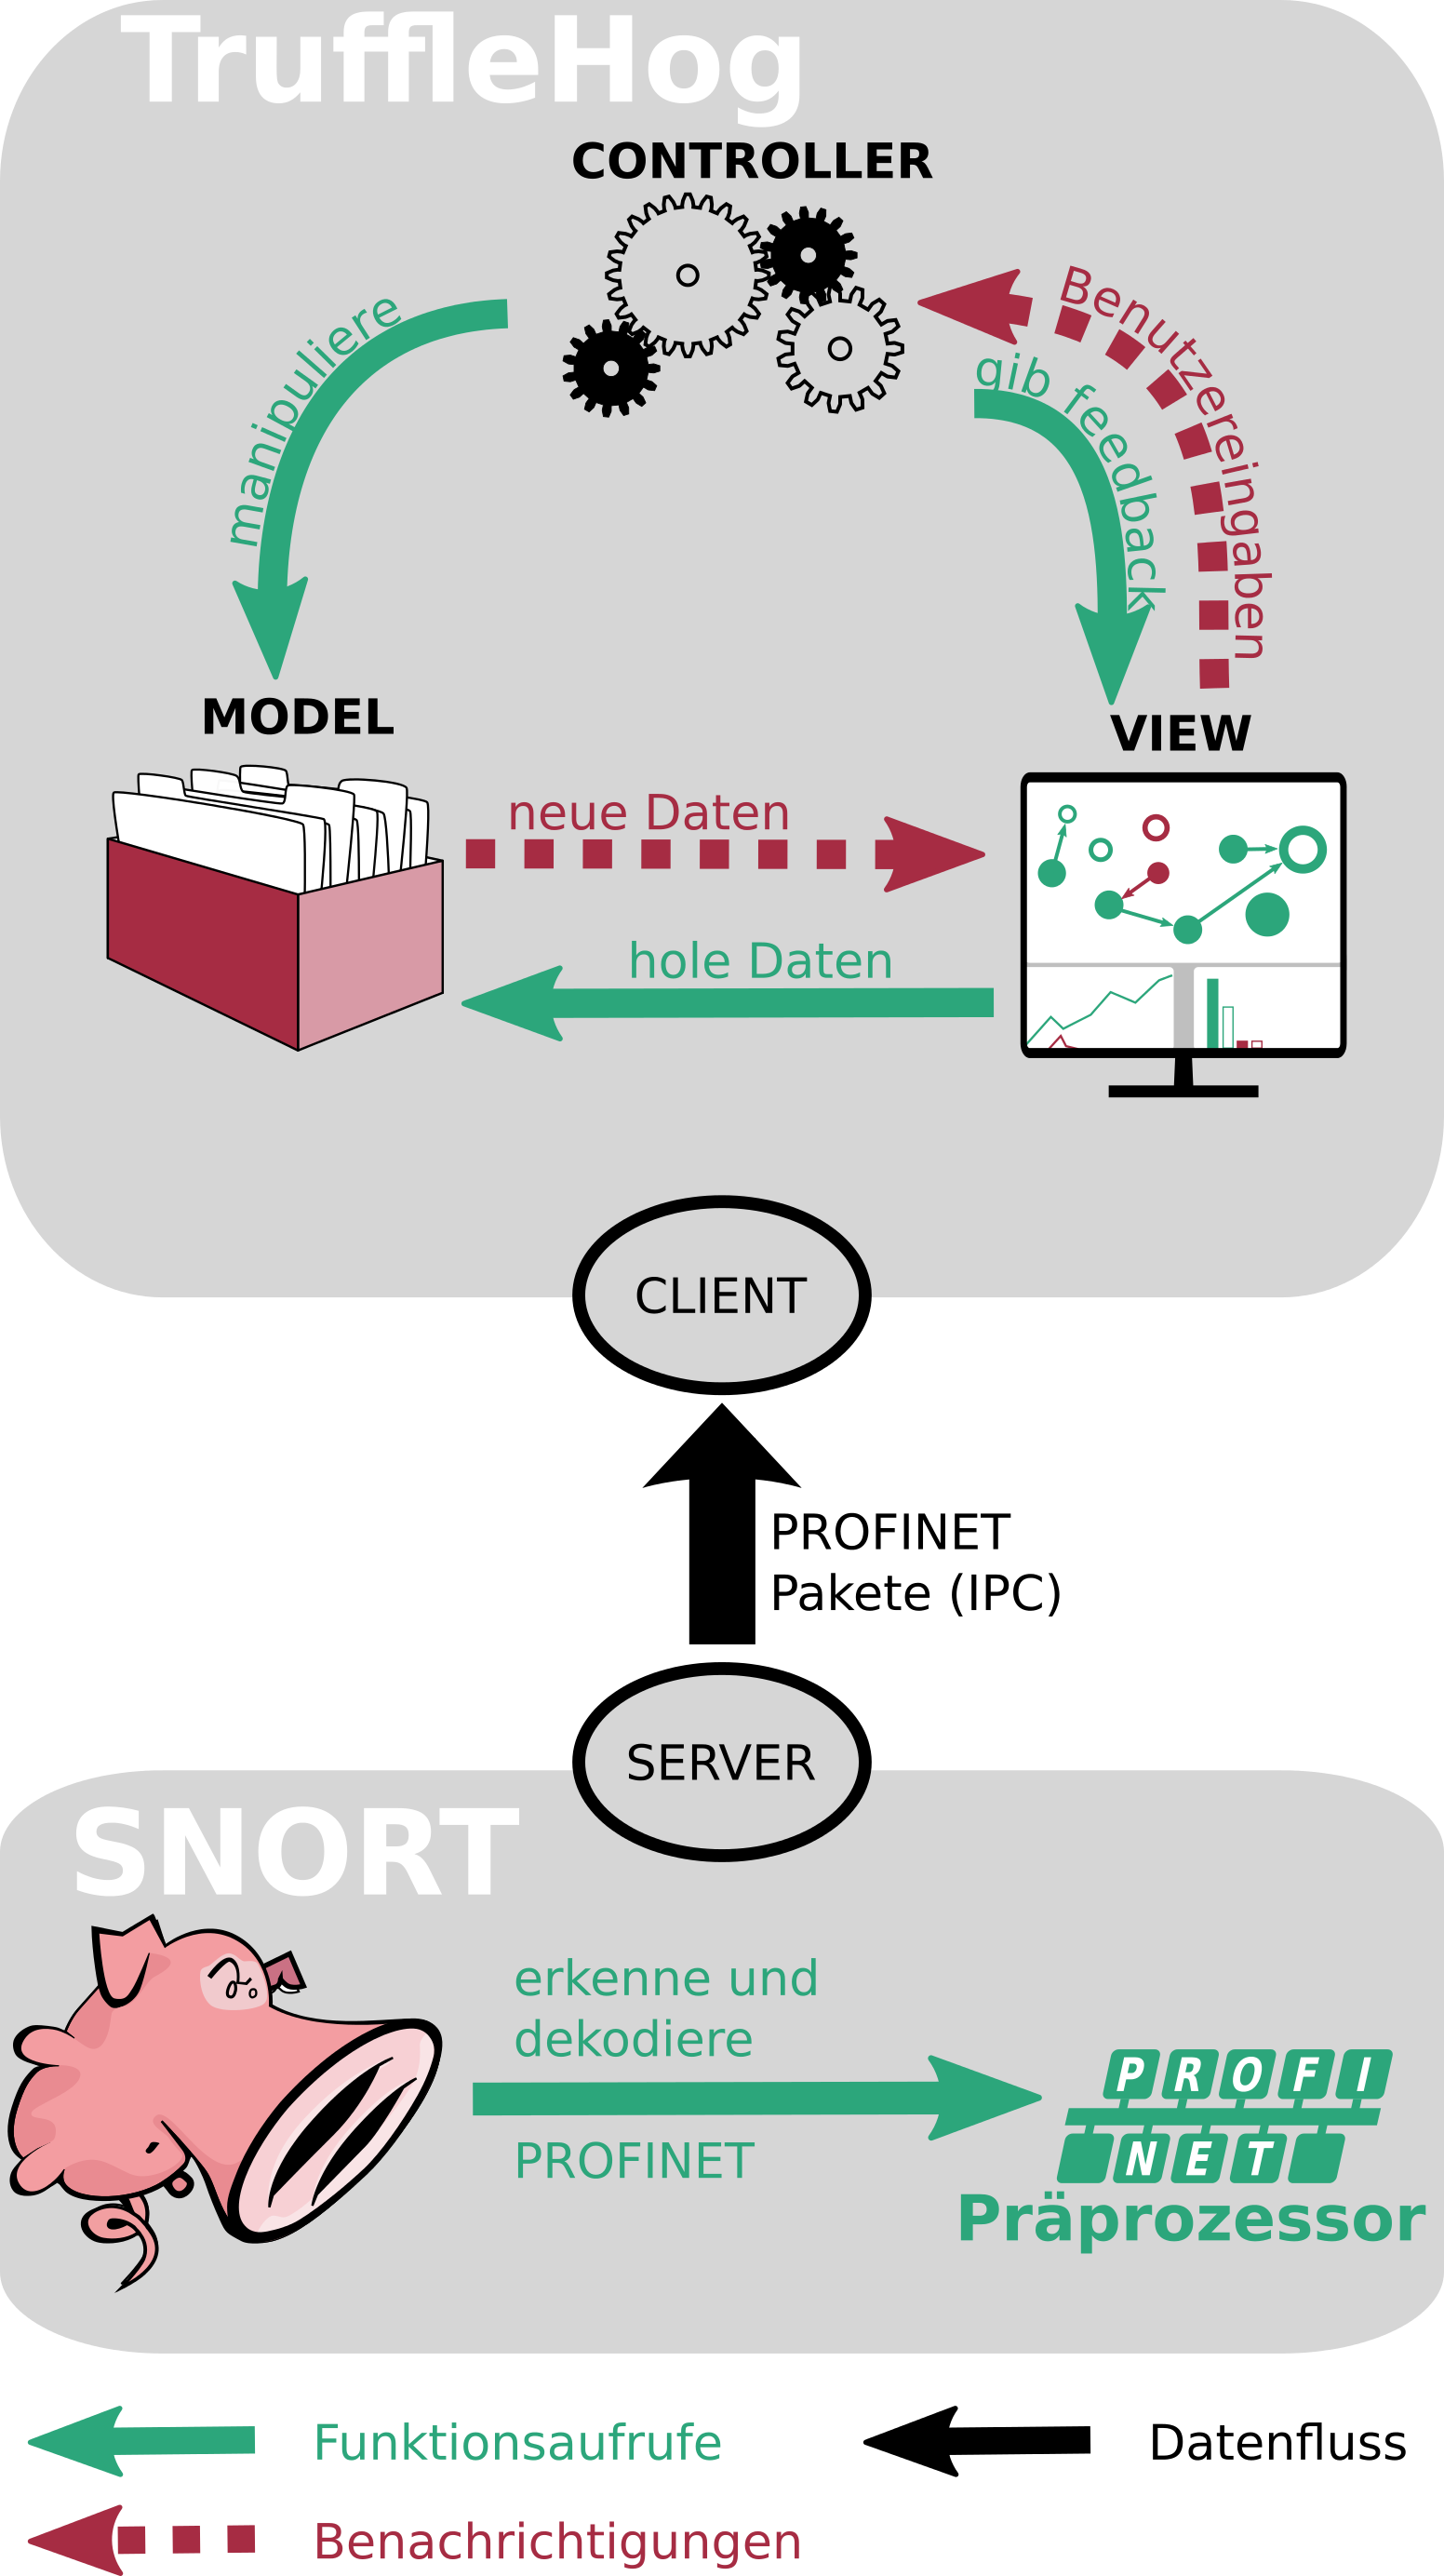
\includegraphics[height=0.9\textheight]{./images/intro_diagram.png}
    \end{figure}
\end{frame}


\section{Snort-Präprozessor}
\begin{frame}{Snort-Präprozessor}
    \begin{itemize}
      \item In Snort verankert
      \pause
      \item Dekodiert Ethernet PROFINET Protokolle wie z.B. DCP oder RT1-3
      \pause
      \item Optional: Auslösen von Alerts im Präprozessor.
    \end{itemize}
\end{frame}


\section{TruffleHog}
\begin{frame}{TruffleHog}
    \begin{itemize}
      \item Auswertung der Paketdaten
      \pause
      \item Visualisierung als Netzwerkgraph
      \pause
	  \item Statistische Auswertung von Kerndaten
    \end{itemize}
\end{frame}

\begin{frame}
	\begin{figure}
		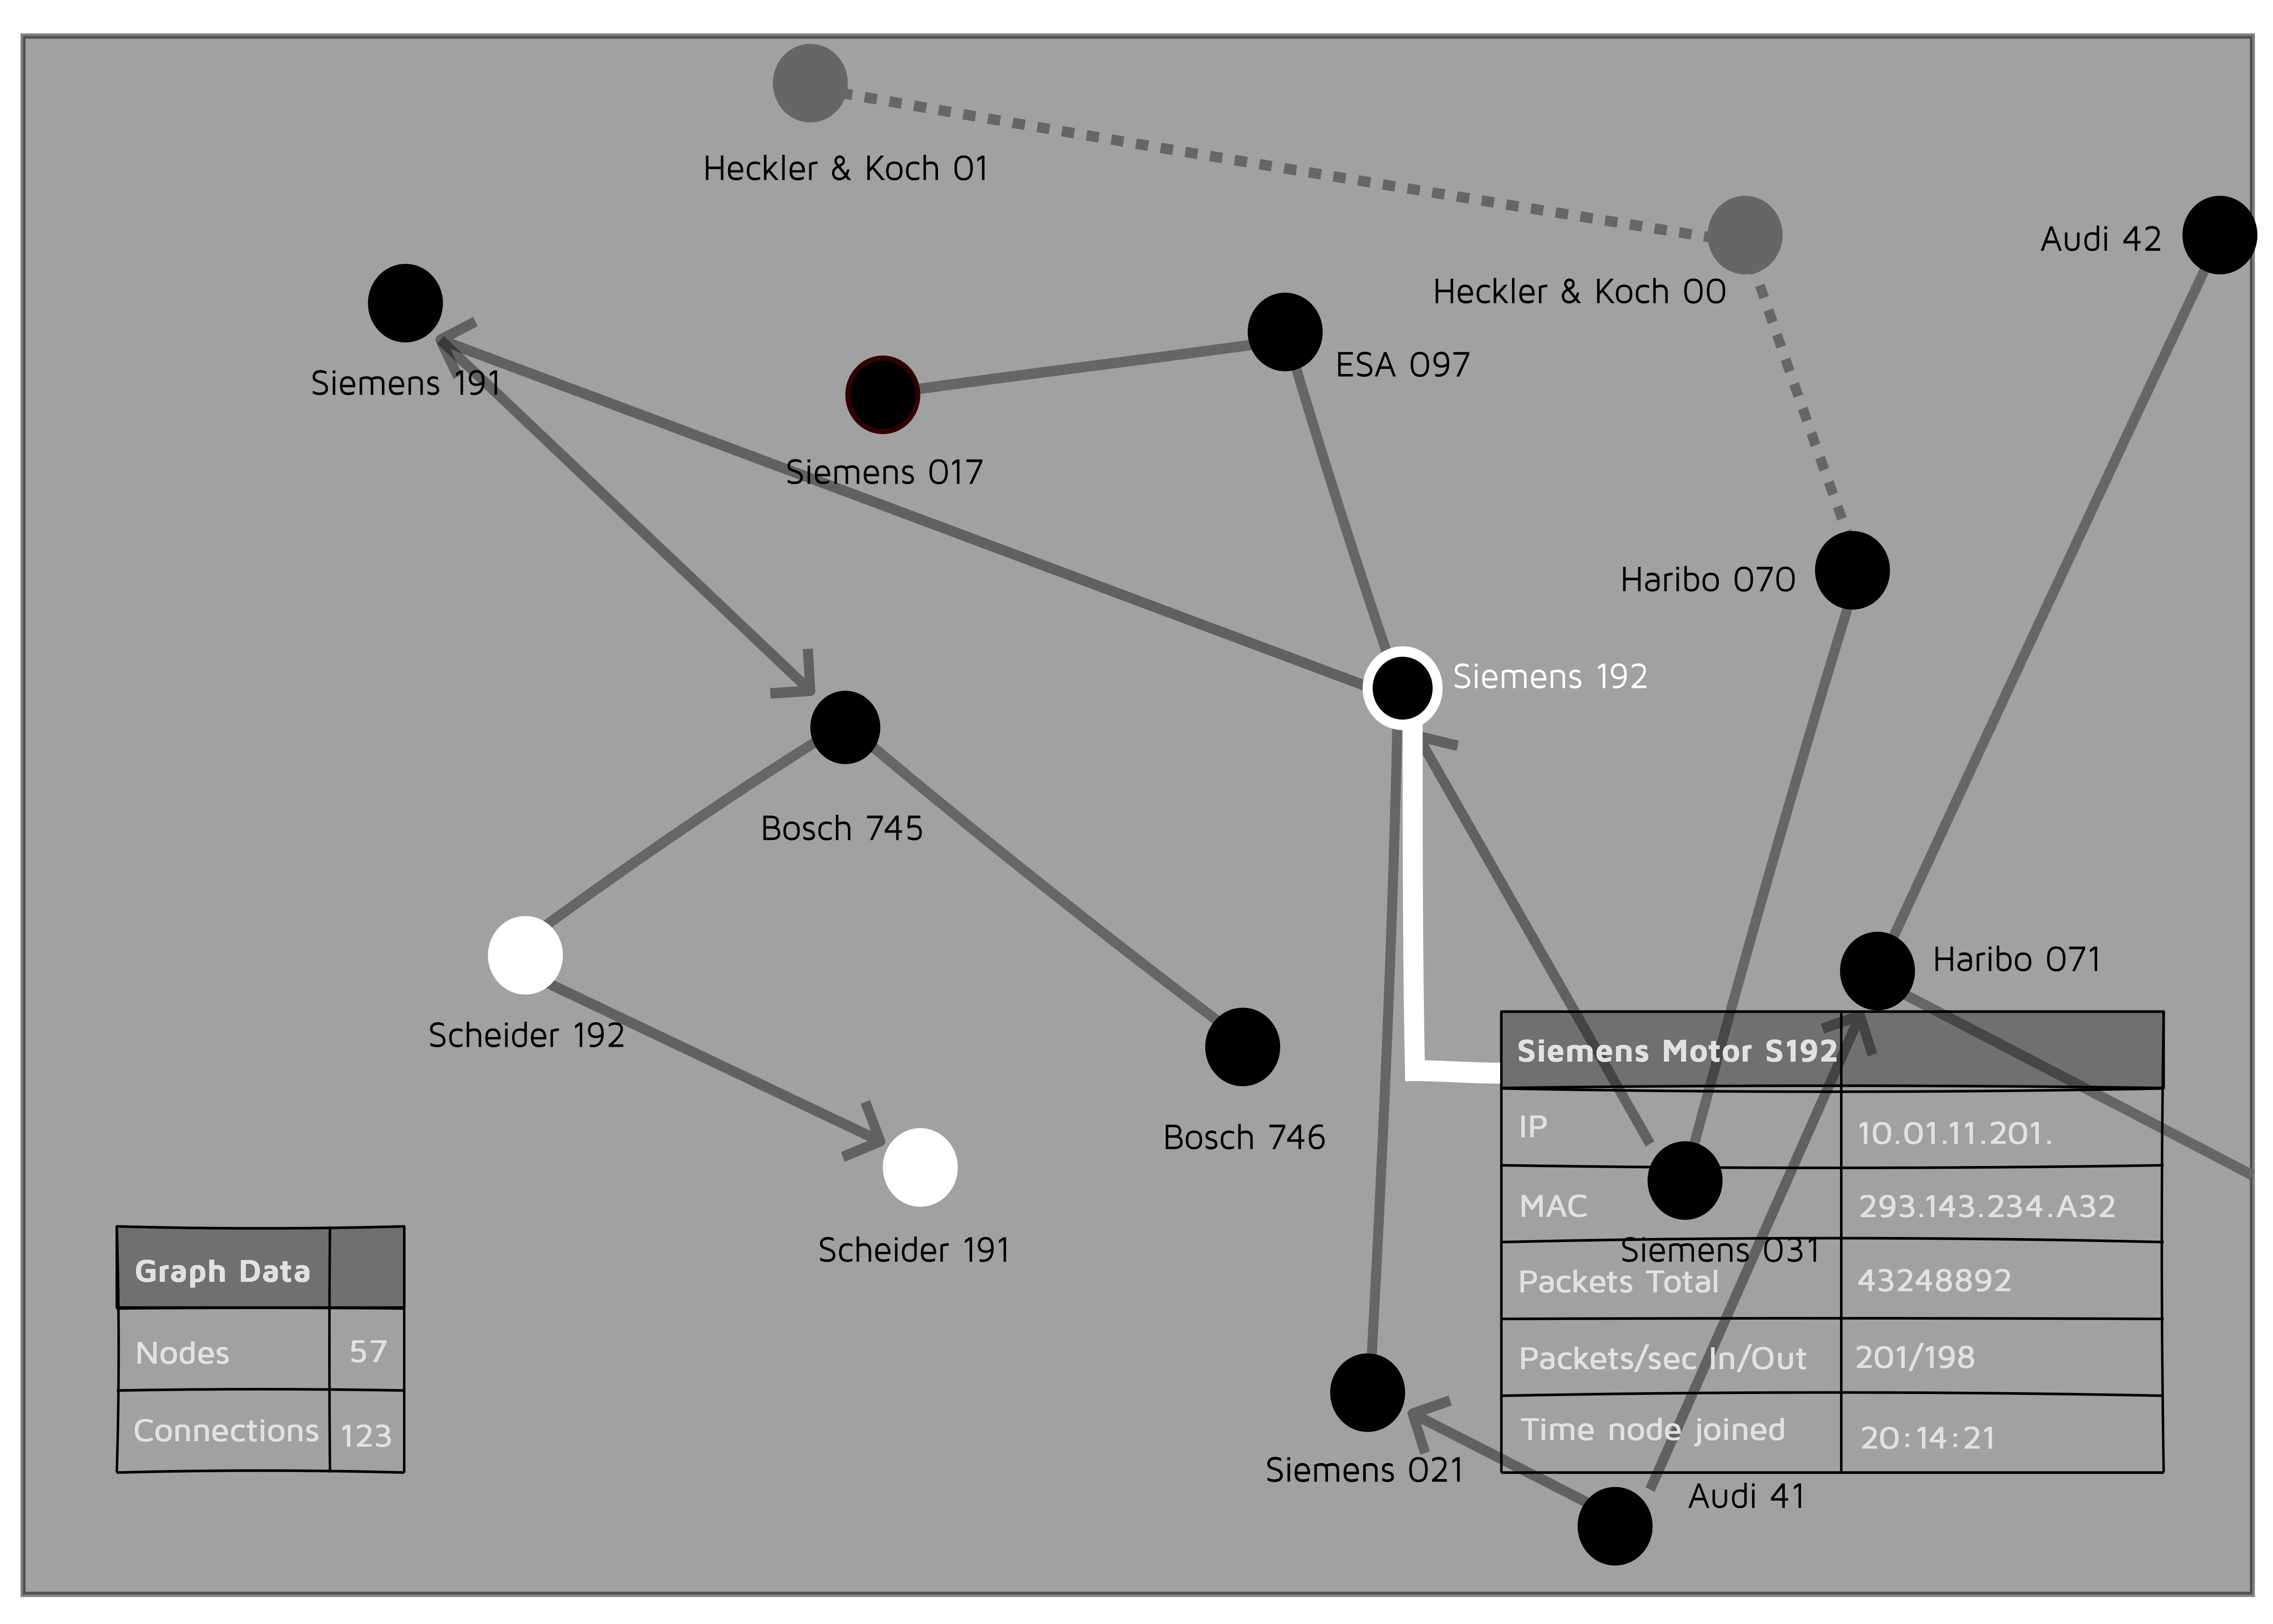
\includegraphics[height=0.95\textheight]{./images/GUI.png}
	\end{figure}
\end{frame}

\section{Zeitplan}
\begin{frame}{Zeitplan}
    \begin{figure}
      \centering
      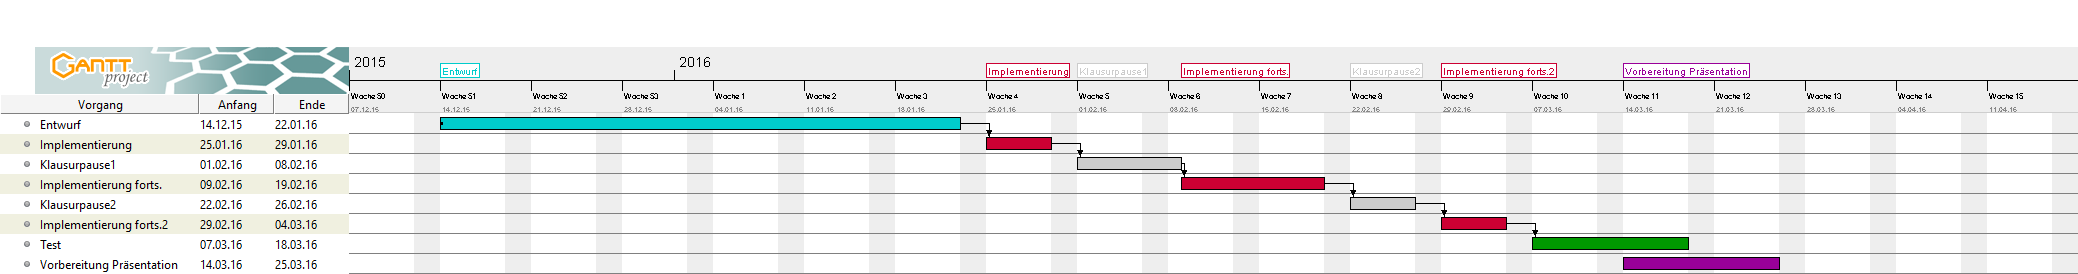
\includegraphics[width=\textwidth]{./images/document.png}
    \end{figure}
\end{frame}

\appendix
\beginbackup

%\begin{frame}[allowframebreaks]{References}
%\printbibliography
%\end{frame}

\backupend

\end{document}
